\documentclass{standalone}
\usepackage{tikz, xcolor, graphicx}
\usetikzlibrary{shapes.geometric, positioning}

\pagestyle{empty}

\begin{document}

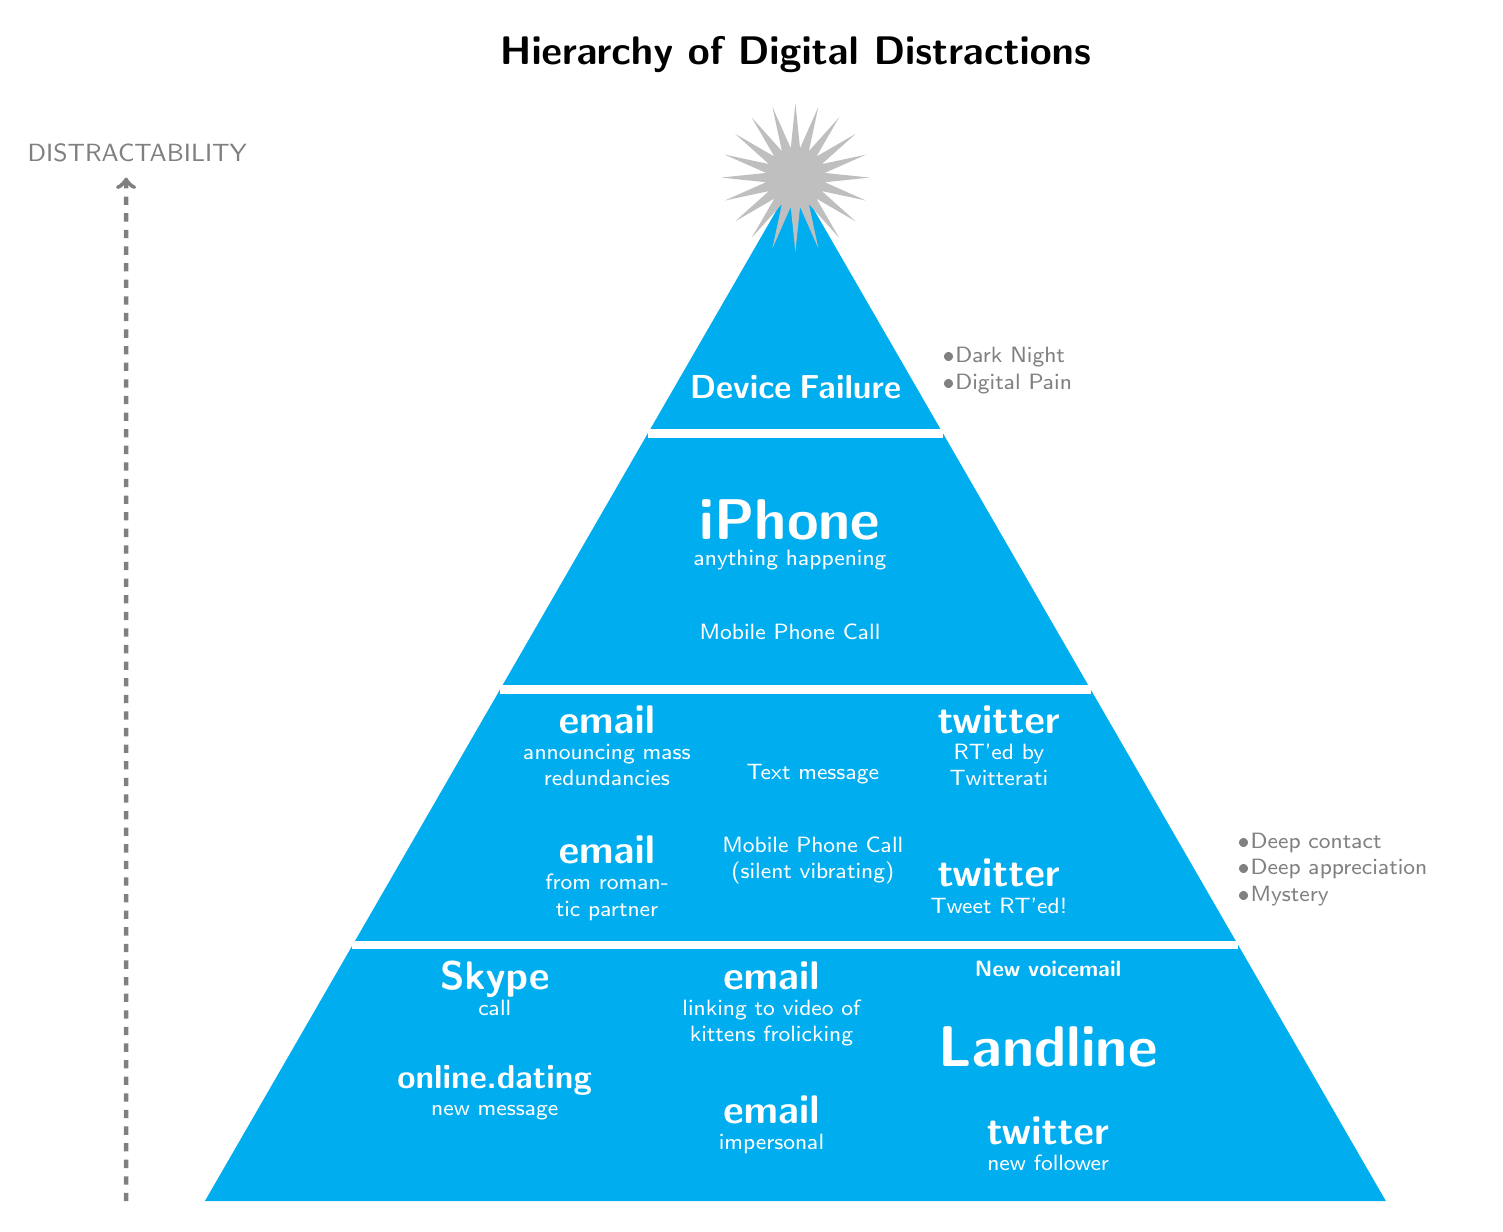
\begin{tikzpicture}[
  font=\footnotesize\sffamily,
  every node/.style={align=center, text=white},
  nobox/.style={draw=none, fill=none, text width=#1, inner sep=0pt}]

% Draw equilateral triangle manually
\coordinate (C) at (0,13); % height = sqrt(3) * side/2 for equilateral triangle of side 6
\coordinate (A) at (-7.5,0); \coordinate (B) at (7.5,0);
\fill[cyan] (A) -- (B) -- (C) -- cycle;

%pyramid layers subdivisions at 1/4, 2/4, 3/4 of pyramid height
\coordinate (A1) at (-5.625, 3.25); \coordinate (B1) at (5.625, 3.25); 
\draw[line width=3pt, white] (A1) -- (B1);

\coordinate (A2) at (-3.75, 6.5); \coordinate (B2) at (3.75, 6.5); 
\draw[line width=3pt, white] (A2) -- (B2);

\coordinate (A3) at (-1.875, 9.75); \coordinate (B3) at (1.875, 9.75); 
\draw[line width=3pt, white] (A3) -- (B3);

%Bottom Layer
\node[nobox=3.4cm, anchor=north west] at ([xshift=0.1cm, yshift=-0.2cm]A1) (skype){
\textbf{\Large Skype}\\
call\\ \vspace{2em}
\textbf{\large online.dating}\\
new message
};
\node[nobox=3.4cm, anchor=north west] at ([xshift=0.1cm]skype.north east) (email){
\textbf{\Large email}\\
linking to video of kittens frolicking\\ \vspace{2em}
\textbf{\Large email}\\
impersonal
};
\node[nobox=3.4cm, anchor=north west] at ([xshift=0.1cm]email.north east){
\textbf{New voicemail} \\\vspace{2em}
\textbf{\huge Landline}\\\vspace{2em}
\textbf{\Large twitter}\\
new follower
};

%Second Layer
\node[nobox=2.5cm, anchor=north west] at ([xshift=0.1cm, yshift=-0.2cm]A2) (email2){
\textbf{\Large email}\\
announcing mass redundancies\\ \vspace{2em}
\textbf{\Large email}\\
from romantic partner
};
\node[nobox=2.5cm, anchor=north west] at ([xshift=0.1cm]email2.north east) (text){
\\\vspace{2em}
Text message\\\vspace{2em}
Mobile Phone Call\\
(silent vibrating)
};
\node[nobox=2cm, anchor=north west] at ([xshift=0.1cm]text.north east){
\textbf{\Large twitter} \\
RT'ed by Twitterati \\\vspace{3em}
\textbf{\Large twitter}\\
Tweet RT'ed!
};
\node[nobox=3cm, anchor=south west, text=gray, align=left] at ([yshift=0.5cm]B1) {
\textbullet Deep contact\\
\textbullet Deep appreciation\\
\textbullet Mystery};

%Third Layer
\node[nobox=3.4cm, anchor=north west] at ([xshift=0.1cm, yshift=-0.2cm]A3){
\\\vspace{2em}
\textbf{\huge iPhone}\\
anything happening\\ \vspace{2em}
Mobile Phone Call
};

%Top Layer
\node[nobox=3.4cm, anchor=north] at ([yshift=-2.5cm]C){
\textbf{\large Device Failure}
};
\node[nobox=2cm, anchor=south west, text=gray, align=left] at ([yshift=0.5cm]B3) {
\textbullet Dark Night\\
\textbullet Digital Pain};

% Top Symbol (stylized manually)
\node[star, star points=20, fill=gray!50, star point ratio=2.5, text width=0.3cm] at (C) (star){};

% Left-side label
\node[nobox=2.5cm, anchor=south, text=gray] at ([xshift=-8.5cm, yshift=0.2cm]C) {\small DISTRACTABILITY};
\draw[dashed, line width=1.6pt, gray, ->] ([xshift=-1cm]A) -- ([xshift=-8.5cm]C);

% Title
\node[anchor=south, text=black] at ([yshift=0.2cm]star.north) {\Large \textbf{Hierarchy of Digital Distractions}};

\end{tikzpicture}
\end{document}
